\section{Overview}

It is challenging to extract and track features of large time-varying volume data in parallel. First, although a feature can be extracted partially on a processor using the conventional methods, we need to build the connectivity information of the feature across multiple processors. Such information allows us to obtain the global description of a feature from a set of neighboring processors, and enables more advance operations such as similarity evaluation. Second, such connectivity information can be dynamically changed with feature evolving over time. We need to update and maintain the connectivity of features in an efficient fashion to track highly intermittent phenomena.

%The biggest challenge for tracking large time-varying volumetric data set lies in that, though features can be extracted within individual processors using the conventional methods, they might also span over multiple data blocks, which is unavoidable as the number of processors increases. To extract and trace a feature over a distributed volume data set, we need to build and maintain the connectivity information of the features across multiple nodes. As feature descriptors, such as size, curvature, and velocity, are distributed among processors, connectivity information can facilitate us to obtain the description of a feature from neighboring processors, and also enable more advanced operations such as similarity evaluation.

However, it typically requires intensive data exchanges among processors to build and maintain connectivity information of features, and thus incurs extra communication cost. To address this issue, we adopt the master-slave paradigm~\cite{Chen03realtime}, but design a different strategy. Instead of being sent back to a host, the local connective information is computed and preserved only in the slaves where the correspondent features reside. Hence there is no global connectivity information preserved in the host. The host only serves as an interface to broadcast the criterion of features to the slaves. In this way, the computation of merging local connectivity information is distributed to the slaves. Thus, we can effectively reduce the potential communication bottleneck on the host.

In addition, our approach does not need a global synchronization for gathering all local connectivity information at the host, thus avoiding potentially long computation time caused by features spanning over a large number of nodes. Furthermore, there are no needs to set a barrier to wait for all connectivity information being sent back to the host. Thus, if there exists features that span over a large number of nodes but are not explored by the user, the potentially long computation time for these features will not block the whole process. This makes it ideal for an interactive system, where users can select the features of interest and instantly receive the visual feedback as the features evolves.

%Our implementation uses a similar system structurer that forms the basis of previous work \cite{Muelder2009}. Figure~\ref{fig:system-overview} depicts a high-level overview of the work flow for a single time-step.
%
%\begin{figure}[ht]
%	\centering
%	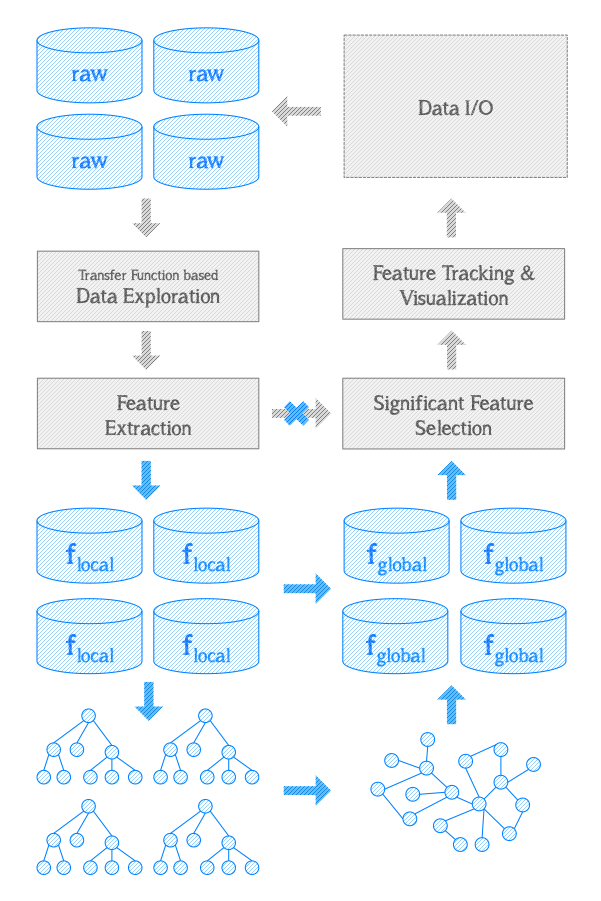
\includegraphics[width=1\linewidth]{system_overview.png}
%	\caption{Work flow of a single time-step}
%	\label{fig:system-overview}
%\end{figure}
%
%First, the source volume data is read either from a pre-generated data set or from a simulation program in-situ. Then, user can identify features of interest via transfer function manipulation as such candidate features will be extracted. However, since the descriptive power of a transfer function is often insufficient to precisely highlight the desired subset of features, user may have to select significant features either by simple point-and-select or iteratively filter out unwanted ones using different feature descriptors. Once the user has identified the interesting features, the system tracks only these significant features in subsequent time steps.
%
%What our approach distinct from that of the previous one lies in that the global connectivity information of each feature need to be obtained before the Significant Feature Selection process could be carried out. As shown in blue color in Figure~\ref{fig:system-overview}, first the raw data are distributed in \textcolor{red}{logically adjacent data blocks.}. After Feature Extraction is done in each data block, the set of local features as well as the local connectivity information will be generated. Then by applying our merging algorithms, global connectivity information can be obtained efficiently such that each data block will possess the global connectivity information for each of its residing features. This enables Signification Feature Selection in a distributed environment and henceforth Feature Tracking and Visualization. 